\begin{frame}
 \titlepage
\end{frame}

\section{Internals}

	\subsection{Git Object Hashmap}
	\begin{frame}[fragile]
	\frametitle{Git Object Hashmap}
	\begin{block}{}
		\begin{itemize}
			\item internal storage git (./.git/objects/)
			\item all content that represents history is stored here, ALL!
			\item stored in a hashmap of sha1 keys to content of objects
			\item different types of objects
		\end{itemize}
	\end{block}

	\begin{lstlisting}
$ git cat-file -p <hash>
	\end{lstlisting}

\note[itemize]{
	\item git history is represented by a series of objects stored in a hashmap
	\item the structure of the repo is represented by having the objects point to the keys of different objects in the hashmap
}
\end{frame}

\begin{frame}[fragile]
	\begin{lstlisting}
$ tree .git/objects
.git/objects/
| 9d/
|   `-- aeafb9864cf43055ae93beb0afd6c7d144bfa4
`-- info/
`-- pack/

3 directories, 1 file
	\end{lstlisting}

\note[itemize]{
	\item Here is where you can find them, they exists on disk
	\item the whole history of the repo is here, on disk,
	\item no network required. (this is why)
}
\end{frame}


	\subsection{Git Objects}
	\begin{frame}
	\frametitle{Git Object Hashmap}

	\begin{columns}
	\begin{column}{0.5\textwidth}
		\begin{itemize}
			\item blob
			\item tree
			\item commit
			\item tag (or are they?)
		\end{itemize}
	\end{column}
	\begin{column}{0.5\textwidth}
		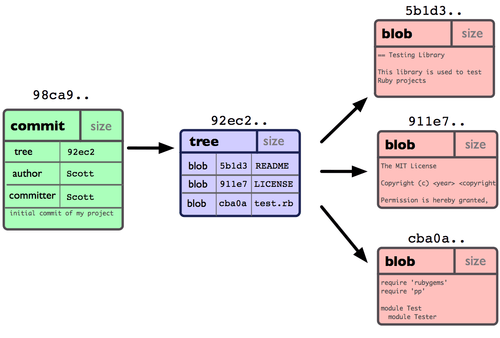
\includegraphics[width=\textwidth]{images/object-types.png}
	\end{column}
	\end{columns}

	\note[itemize]{
		\item all these are compressed
		\item have a tag at the top that tells git what the type is.
		\item blob is flat file copy
	}
\end{frame}

\begin{frame}[fragile]
	\frametitle{blob}

	\begin{columns}
	\begin{column}{0.5\textwidth}
		\begin{itemize}
		\item flat files
		\item the actual source code
		\item full copy
		\item has no further references to other objects
		\end{itemize}
	\end{column}
	\begin{column}{0.5\textwidth}
		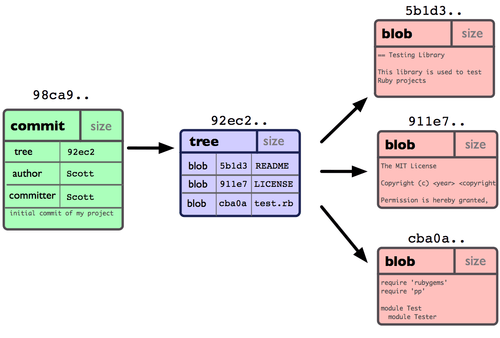
\includegraphics[width=\textwidth]{images/object-types.png}
	\end{column}
	\end{columns}

	\note[itemize]{
		\item blob is flat file copy
	}
\end{frame}

\begin{frame}[fragile]
	\frametitle{tree}

	\begin{columns}
	\begin{column}{0.5\textwidth}
		\begin{itemize}
		\item represents a directory on disk
		\item retains file permissions (in unix notation)
		\item points to other trees and blobs
		\end{itemize}
	\end{column}
	\begin{column}{0.5\textwidth}
		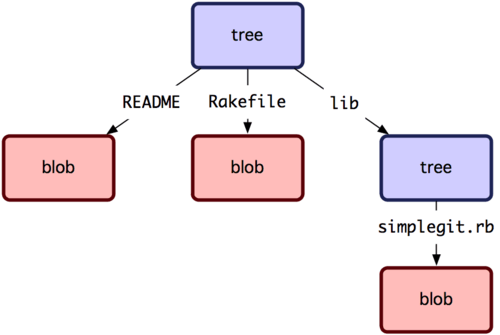
\includegraphics[width=\textwidth]{images/trees.png}
	\end{column}
	\end{columns}

\end{frame}

\begin{frame}[fragile]
	\frametitle{commit}

	\begin{columns}
	\begin{column}{0.5\textwidth}
		\begin{itemize}
		\item stores author, timestamp, message, ...
		\item points to a tree
		\item points to 1 or more commits (parent commits)
		\end{itemize}
	\end{column}
	\begin{column}{0.5\textwidth}
		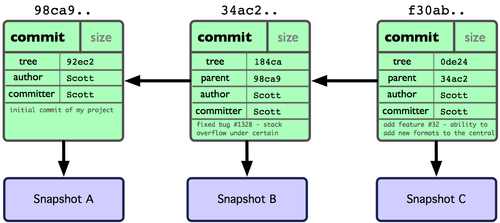
\includegraphics[width=\textwidth]{images/commits.png}
	\end{column}
	\end{columns}

	\note[itemize]{
		\item history is represented solely in commit objects, it has noting to do with
		code, trees, or blobs.
	}
\end{frame}

\begin{frame}
	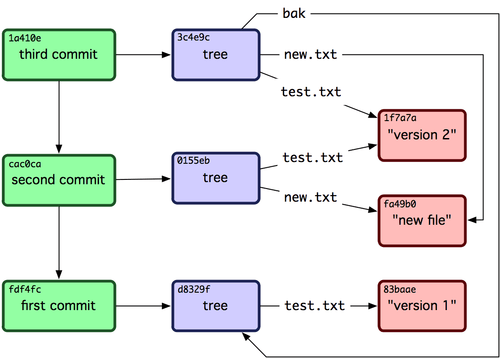
\includegraphics[width=\textwidth]{images/git-objects.png}
\end{frame}


	\subsection{branches are not objects, what is head}
	\begin{frame}
	\frametitle{branches}

	\begin{block}{}
		\begin{itemize}
			\item point to a commit (flat file with sha1 hash).
			\item moves pointer on commit, revert, rebase, reset, ...
			\item stored in .git/refs/
		\end{itemize}
	\end{block}
\end{frame}

\begin{frame}
	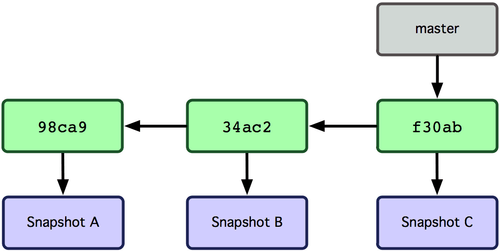
\includegraphics[width=\textwidth]{images/branches.png}
\end{frame}

\begin{frame}
	\frametitle{What is HEAD}

	\begin{block}{}
		\begin{itemize}
			\item points to a branch
			\item flat file with relative path to branch
			\item or sha1 hash in detached head mode.
			\item moves on git checkout
			\item does NOT move on revert, rebase, reset, commit, ...
		\end{itemize}
		\note[itemize]{
			\item `\$ git checkout head~ && cat .git/HEAD` (detached)
		}
	\end{block}
\end{frame}

\begin{frame}
	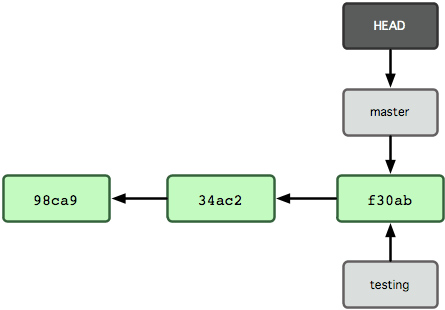
\includegraphics[width=\textwidth]{images/head.png}
\end{frame}



	\subsection{tags}
	\begin{frame}
	\frametitle{Tags vs Anotated Tags}

	\begin{block}{Tags}
		\begin{itemize}
			\item comparable to branch, can not be commit on
			\item located in .git/refs/tags
			\item does not create git objects
		\end{itemize}
	\end{block}

	\begin{block}{Anotated Tags}
		\begin{itemize}
			\item comparable to branch, can not be commit on
			\item has tagger, time and message
			\item can be cryptographically signed! (REAL TAGS)
			\item does create git objects (`git cat-file -p <tag-name>`)
			\item will be used for releases.
		\end{itemize}
	\end{block}

\end{frame}


	\subsection{demo}
	\begin{frame}
	\begin{block}{}
		\begin{center}
			Demo
		\end{center}
	\end{block}
\end{frame}



\section{Cases}

	\input{./slides/revert.tex}
	\input{./slides/rebase.tex}

\section{Interactive}

% -- \begin{frame}
% -- 	\begin{itemize}
% -- 		% Begin met bestaande repo, live clone?
% -- 		\item toon .git/objects
% -- 		\item pack file + info file
% -- 		\item git add voegt file toe in objects (niet on commit, on add)
% -- 		\item git staging
% -- 		\item `git gc` (files toegevoegd zijn WEG, oh noez)
% -- 		\item git commit voegt tree bij en commit bij
% -- 			- branch moves forward (`cat .git/refs/heads/branch-name`)
% -- 		\item merge
% -- 			- toon dat `git cat-file -p commit-hash` meerdere parents heeft
% -- 			- contrast `git cat-file -p non-merge-commit-hash`
% -- 			- octoppus merges
% -- 			- ORDE IS BELANGRIJK, kijk welke branch moved.
% -- 			- (side note ook u hash gaat anders zijn.)
% -- 		\item references naar commits (head~ head~n, head\^, head\^2)
% -- 			- chainable (head~\^2~3) (tree-ish)
% -- 		\item reflog
% -- 			- haal 'verloren' \{commits,files, ...\} terug,
% -- %			- head@{1}, branch@{1}, branch@{two days ago}
% -- %		\item remotes (origin no clone), tracking branches.
% -- %			- (git branch --set-upstream-to=origin/remote-branch-name)
% -- %			- git push remote local-branch-name:remote-branch-name
% -- %			- git fetch \&\& git checkout branch-name # remote heeft branchname,
% -- %			  dan branch tracked remote automatische.
% -- %			- git fetch -p || git fetch --prune (als remote tracking branch verwijdern,
% -- %			  local ook)
% -- %		\item multiple remotes
% -- 	\end{itemize}
% -- \end{frame}


\section{Gitflow}
	\begin{frame}
	\frametitle{gitflow}
	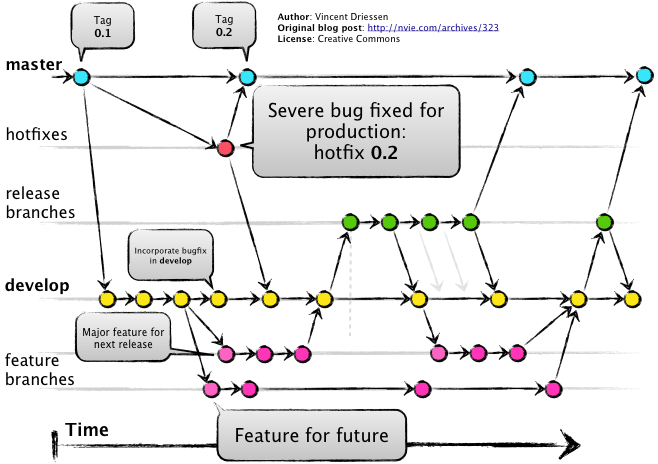
\includegraphics[width=\textwidth]{images/gitflow.png}
\end{frame}

\begin{frame}
	\frametitle{gitflow branches}
	\begin{block}{}
	\begin{itemize}
		\item master, develop (ever present)

		\item feature branch (each jira ticket)
		\item hotfix branch (production issues)
		\item release branch (only showstopper)
	\end{itemize}
	\end{block}
\end{frame}

\begin{frame}
	\frametitle{gitflow rules}
	\begin{block}{}
	\begin{itemize}
		\item feature branch:
		\begin{itemize}
			\item from develop
			\item to develop
		\end{itemize}

		\item hotfix branch:
		\begin{itemize}
			\item from master
			\item to master and develop (develop will also need this fix)
		\end{itemize}

		\item release branch:
		\begin{itemize}
			\item from develop
			\item to master and develop
		\end{itemize}
	\end{itemize}
	\end{block}
\end{frame}


	\subsection{Scenarios}
	\begin{frame}
	\frametitle{You are implementing a feature.}

	\begin{block}{}
	\begin{itemize}
		\item create branch ('feature/JIRA-547')
		\item commit, commit, commit, ..., revert, commit again
		\item keep running unit tests
		\item create pull request
		\item reviewer merges back into develop
		\item ci deploys develop to TST
	\end{itemize}
	\end{block}
\end{frame}

\begin{frame}
	\frametitle{feature pull request breaks CI build}

	\begin{block}{}
	\begin{itemize}
		\item merge develop in feature/JIRA-547
		\item commit, commit, commit, ... (hopefully fixing stuff)
		\item reopen pull request
		\item rinse and repeat
	\end{itemize}
	\end{block}
\end{frame}

\begin{frame}
	\frametitle{Preparing for a new release}
	\begin{block}{}
	\begin{itemize}
		\item branch from develop ('release/release-version')
		\item deploy release branch to ACC
		\item have customer test everything
		\item fix showstoppers on release branch
		\item merge into master and back into develop
		\item tag merge commit on master branch
	\end{itemize}
	\end{block}
\end{frame}

\begin{frame}
	\frametitle{Production goes down}
	\begin{block}{}
	\begin{itemize}
		\item branch from master ('hotfix/issue-description')
		\item commit, commit, commit, ...
		\item merge into master and develop
		\item tag merge commit on master branch
		\item deploy master to PRD
	\end{itemize}
	\end{block}
\end{frame}


	\subsection{demo}
	\begin{frame}
	\begin{block}{}
		\begin{center}
			Demo
		\end{center}
	\end{block}
\end{frame}


	\subsection{previous encountered issues}
	\begin{frame}
	\frametitle{merge vs rebase}
	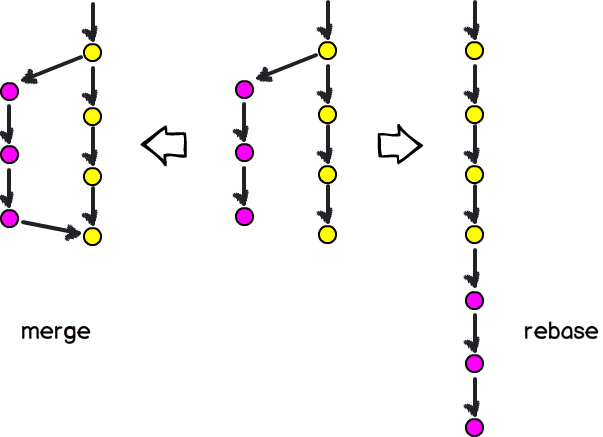
\includegraphics[width=\textwidth]{images/merge-vs-rebase.png}
\end{frame}

	\begin{frame}
	\frametitle{interesting links}

	\begin{block}{}
		\begin{itemize}
			\item Knowledge is Power: Getting out of trouble by understanding Git by Steve Smith
			\item \url{www.youtube.com/watch?v=sevc6668cQ0}
		\end{itemize}
	\end{block}
\end{frame}

